\textbf{Single Responsibility Principle}

There are various manifestations of \gls{srp} implemented in the artifacts. One of which is
already mentioned in Figure \ref{fig_modulair_components}, where \gls{srp} is applied to
separate the domain logic from the application, infrastructure and presentation logic. One
could argue that this manifestation is more related to \gls{soc}, considering the high
granularity of the components.

A better example is the separation of handlers that are part of the \gls{ca}
Expander. Each of those handlers executes an isolated part of the expanding process.
Consider the Listing \ref{list_entityexpander} \nameref{list_entityexpander}
\parencite{koks_expandentitieshandlerinteractor_2023} for example. This Handler is solely
responsible for the generation of data entities. 

\begin{figure}[H]
    \centering
    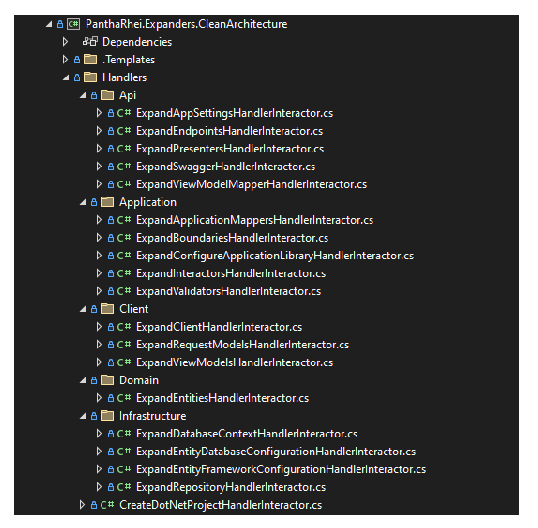
\includegraphics[width=0.6\textwidth]{figures/expander_handlers.pdf}
    \caption[handlers]{Each of the handlers handles an isolated part of the expanding process.}
    \label{fig_handlers}
\end{figure}

\lstinputlisting[
    caption={The \citetitle{koks_expandentitieshandlerinteractor_2023}},
    label={list_entityexpander}]
    {Snippets/ExpandEntitiesHandlerInteractor.cs}

    \textbf{Open/Closed Principle}
    
A relevant manifestation of \gls{ocp} are all the different implementations of expander
handlers in figure \ref{fig_handlers}. The availability of the
\code{koks_iexpanderhandlerinteractor_2023} interface makes it possible to add more
functionality to the CleanArchtictureExpander without modifying any existing
implementation. New handlers are added by extension, and when implemented correctly, the
handler is automatically executed in the desired order and the required conditions.

\lstinputlisting[
    caption={The \citetitle{koks_iexpanderhandlerinteractor_2023}},
    label={list_iexpanderhandlerinteractor} ]
    {Snippets/IExpanderHandlerInteractor.cs}

\lstinputlisting[
    caption={The \citetitle{koks_iexecutioninteractor_2023}},
    label={list_iexecutioninteractor} ]
    {Snippets/IExecutionInteractor.cs}

The fact that \citecode{koks_iexpanderhandlerinteractor_2023} derives from
\citecode{koks_iexecutioninteractor_2023} is another manifestation of \gls{ocp}. This
design decision allows for object types that need to be treated as executables by the
\code{koks_codegeneratorinteractor_2023}. Examples are
\citecode{koks_regionharvesterinteractor_2023},
\citecode{koks_regionrejuvenatorinteractor_2023},
\citecode{koks_preprocessorinteractor_2023} and
\citecode{koks_postprocessorinteractor_2023}. 

Listing \ref{list_CodeGeneratorInteractor} shows the
\code{koks_codegeneratorinteractor_2023} that cohesively executes all of the
\code{koks_iexecutioninteractor_2023} in order. The software engineer only has to focus on
implementing the specific type of \code{koks_iexecutioninteractor_2023} without having to
affect the implementation. This is by definition an example of \enquote{open for
extension} and \enquote{closed for modifications}.

\textbf{Liskov Substitution Principe}

The practical implications of \gls{lsp} are many. In software design, we should strive to
create subtypes that are as similar as possible to their base types in terms of their
behavior and the constraints they impose. In testing, it means that we should test
subtypes to ensure that they behave correctly when used in place of their base types.

Consider \citecode{koks_abstractexpander_2023}. This (abstract) object type allows for
multiple implementations of \textit{Expanders}. The primary example is the
\citecode{koks_cleanarchitectureexpander_2023} which is responsible for generating the
expanded artifact that is part of this research. Different types of expanders could be
added to the generator, ensuring they all behave in the same way.

The \citecode{koks_icreategateway_2023} in Listing \ref{list_icrreategateway} is another
example. The artifact has two implementations of this interface. The data of the entities
are currently stored in the database, but harvest data is serialized to XML using the same
\code{koks_icreategateway_2023} interface. With this design decision, it is very easy to adapt
to a different type of storage mechanism if future requirement demand such a change.

One might notice the similarities with the \gls{ocp}. The difference is that the \gls{ocp}
focuses on the extensibility of the system, without having to modify existing code.
\gls{lsp} ensures that the behavior of different subtypes is following the required
functionality. \gls{lsp} supports \gls{ocp}, but it is not the only way of doing so.

\lstinputlisting[
    caption={The \citetitle{koks_icreategateway_2023}},
    label={list_icrreategateway} ]
    {Snippets/ICreateGateway.cs}

\lstinputlisting[
    caption={The \citetitle{koks_genericrepository_2023} and \citetitle{koks_harvestrepository_2023}},
    label={list_icrreategatewayImplementations} ]
    {Snippets/ICreateGatewayImplementations.cs}

